Monoblocks in a fusion reactor will be exposed to a wide range of exposure conditions (heat and particle fluxes) and their behaviour in terms of hydrogen transport will change based on these conditions.
In ITER, these fluxes can reach $\approx$ \SI{10}{MW.m^{-2}} and $\approx$ \SI{e24}{H.m^{-2}.s^{-1}} (see \reffig{divertor exposure conditions}).
The distribution of these fluxes depend on many operation parameters.

One way of simulating a whole divertor would be to simulate each and every monoblock for a given scenario along one Plasma-Facing Unit.
However, this method would be computationally expensive as it requires redoing the simulations for every scenario.

Another, more efficient method, is to perform a parametric study on a monoblock.
The exposure parameters are varied and for each set of parameters, the quantity of interest (here the hydrogen inventory) is computed.
A relationship is then produced between the exposure parameters and the quantity of interest: a \textit{behaviour law}.
This method is more robust in the sense that it does not require to run additional simulations once this relationship is obtained but simply uses this relationship to obtain the quantity of interest.

The goal of this Section is to establish this relationship between the exposure conditions of the monoblock and its hydrogen content at a given time.

\subsection{Assumptions and simplifications}

For the sake of simplicity and computational time, Trap 2 (in W) is neglected.
Note that this method could be applied to any set of trapping parameters.
Continuity of mobile concentration at interfaces between materials is also assumed in order to save computational time (see \refsec{influence of interface conditions}).
To remain conservative, no recombination on the gaps (toroidal and poloidal) is assumed.
The 2D approximation can therefore be used (see \refsec{influence of dimensionality}).
Moreover, cycling is neglected (see \refsec{influence of cycling}).
The temperature will be imposed on $\Gamma_\mathrm{top}$ from the relationship obtained in \refsec{monoblock thermal behaviour}.


\subsection{Results}

In this section, the total inventory of hydrogen in monoblocks has been calculated as a function of $T_\mathrm{surface}$ and $c_\mathrm{surface}$.
Temperature and mobile concentration of hydrogen were imposed with Dirichlet boundary conditions on $\Gamma_\mathrm{top}$ with $T_\mathrm{surface}$ varying from $T_\mathrm{coolant}$ to \SI{1200}{K} and $c_\mathrm{surface}$ varying arbitrarily from \SI{e20}{m^{-3}} to \SI{6e22}{m^{-3}}.
For surface temperatures below \SI{500}{K}, 1D simulations were performed for the penetration depth of hydrogen remained very low (a few microns) and 1D approximation was sufficient \sidecite{benannoune_numerical_2019}.
For temperatures above \SI{500}{K} for which edge effects become dominant, 2D simulations have been performed.

After $ \SI{e7}{s}$ a high retention zone appeared far from the exposed surface $\Gamma_\mathrm{top}$ (see \reffig{retention fields}).
This high retention zone is due to thermal effects.
As seen in \reffig{T field 1 MW} and \reffig{T field 10 MW}, the temperature was found to decrease in regions close to the cooling pipe $\Gamma_\mathrm{coolant}$ leading to an increase in trap occupancy, creating this high retention zone.
This is however not true for monoblocks where $T_\mathrm{surface} \approx T_\mathrm{coolant}$ since the temperature gradient in the domain is very low.
Instead, trap occupancy is close to one and the retention is high in the whole region where hydrogen has penetrated and not only far from the top surface.

\begin{figure*}
    \centering
    \begin{subfigure}{0.5\linewidth}
        \centering
        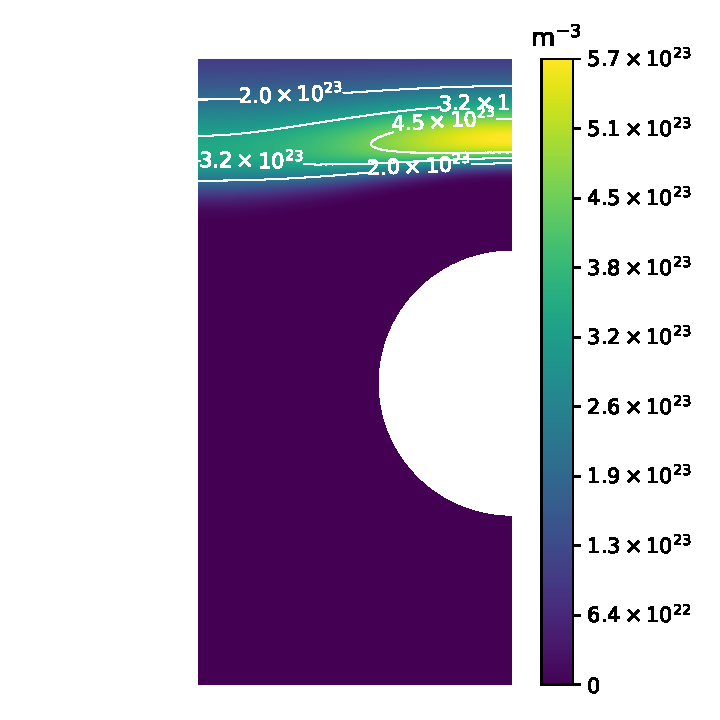
\includegraphics[height=\linewidth]{Figures/Chapter3/monoblocks/parametric_study/retention_T=7.000e+02;c=1.00e+20.pdf}
        \caption{$T_\mathrm{surface} = \SI{700}{K}$ and $c_\mathrm{surface} = \SI{e20}{m^{-3}}$.}
    \end{subfigure}%
    \begin{subfigure}{0.5\linewidth}
        \centering
        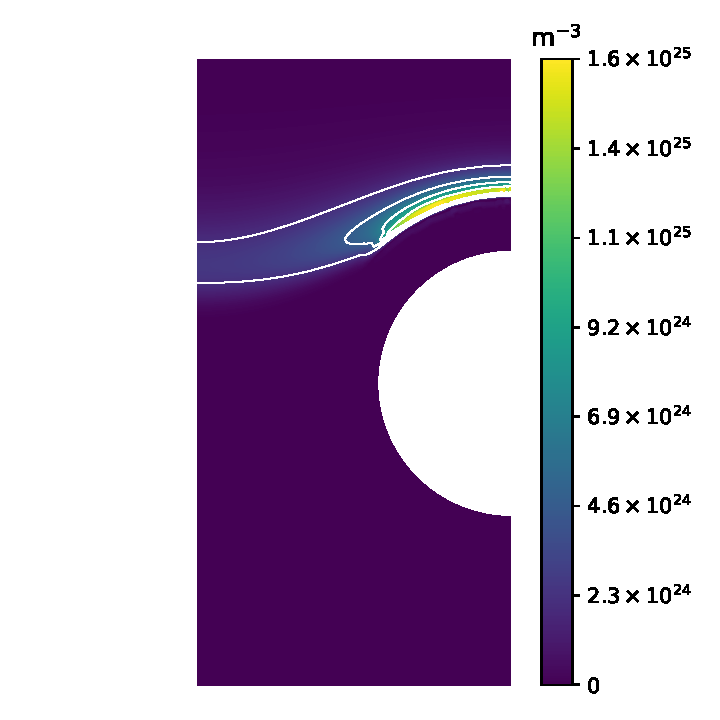
\includegraphics[height=\linewidth]{Figures/Chapter3/monoblocks/parametric_study/retention_T=1.000e+03;c=1.00e+21.pdf}
        \caption{$T_\mathrm{surface} = \SI{1000}{K}$ and $c_\mathrm{surface} = \SI{e21}{m^{-3}}$.}
    \end{subfigure}
    \caption{Example retention fields in \si{m^{-3}} after a \SI{e7}{s} exposure.}
    \labfig{retention fields}
\end{figure*}


In order to obtain this continuous field (see \reffig{inventory T c}), more than 600 simulations randomly distributed on the parameter plane were run and analysed using a Gaussian process machine learning algorithm \sidecite{rasmussen_gaussian_2006} as in \sidecite{shimwell_multiphysics_2019} based on the python package inference-tools \sidecite{chris_bowman_c-bowmaninference-tools_2020}.
The inventory obtained by the Gaussian regression process is also given for a constant value of $c_\mathrm{surf}=\SI{2e21}{m^{-3}}$ (top inset) and a constant temperature $T=\SI{850}{K}$ (left inset).
The Gaussian regression process was particularly appropriate as it calculates a local standard deviation $\sigma$ based on the localisation of the data points and the deviation of the computed inventories.
The lower the density of simulation points, the higher was the value of $\sigma$ (for example around \SI{850}{K} on the top inset of \reffig{inventory T c}).
However, despite the lack of simulation in this region, the value of $\sigma$ was still acceptable (only a few percents of the inventory) ensuring the quality of the resulting interpolation.

As expected, inventory was found to globally increase with $c_\mathrm{surface}$.
For $T_\mathrm{surface} > \SI{550}{K}$, the inventory tended to decrease with surface temperature.
However, for $T_\mathrm{surface} < \SI{550}{K}$, inventory increased with surface temperature.
This phenomenon is due to a trade-off between an increase of the detrapping rate and an increase of the diffusion coefficient making the hydrogen particles penetrate deeper into the bulk.
Above $\SI{550}{K}$, detrapping becomes dominant and inventory decreases.
This mapping of inventory as a function of $T_\mathrm{surface}$ and $c_\mathrm{surface}$ provides an easy way of estimating the inventory in monoblocks for several exposure conditions without having to run many simulations.
Indeed, to estimate the inventory with different exposure conditions, one only needs to associate these conditions $(\varphi_\mathrm{inc}, E)$ to a couple $(c_\mathrm{surf}, T_\mathrm{surf})$.

\begin{figure*} [h]
    \centering
    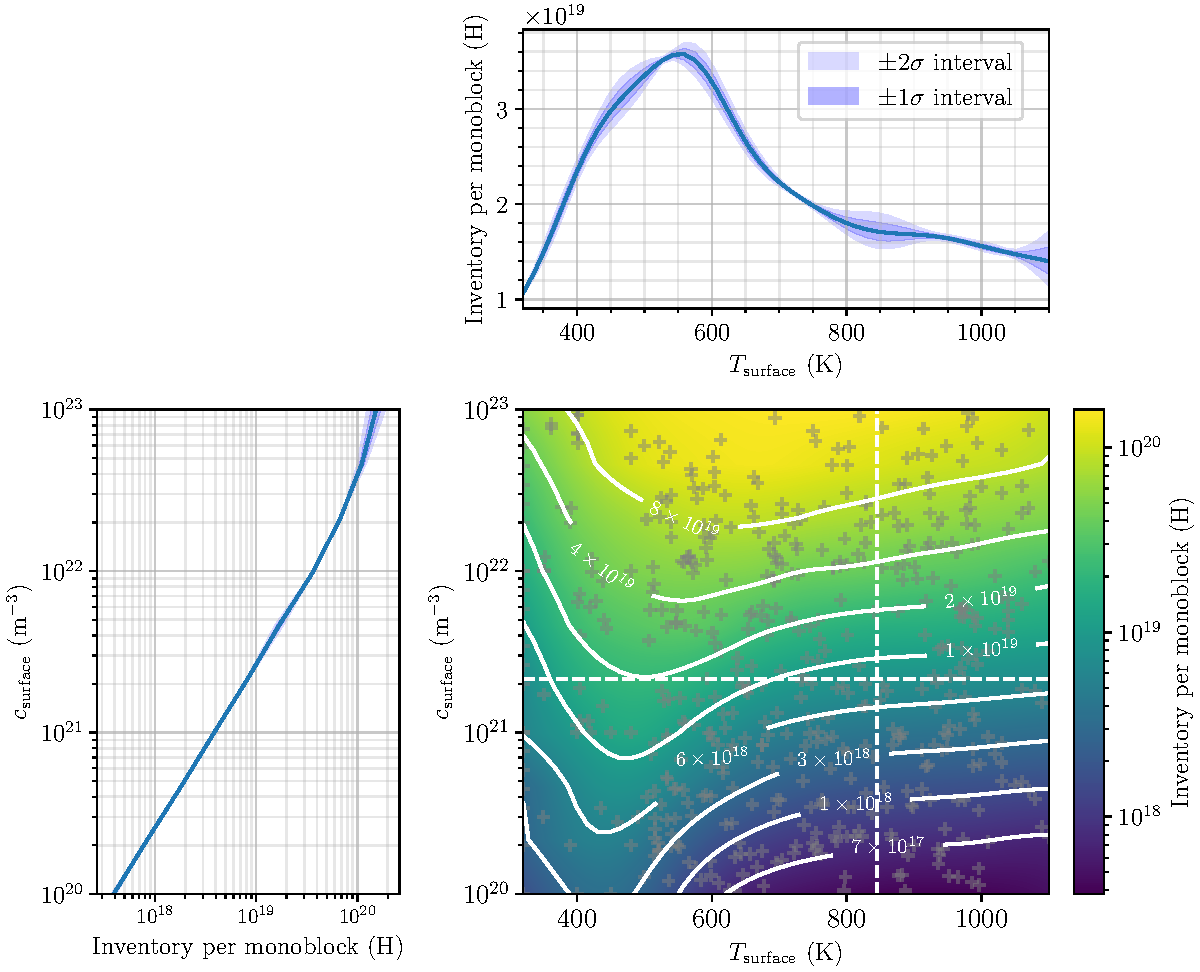
\includegraphics[width=\linewidth]{Figures/Chapter3/monoblocks/parametric_study/inventory_T_c_profiles.pdf}
    \caption{Evolution of the inventory after a \SI{e7}{s} exposure as a function of $T_\mathrm{surface}$ and $c_\mathrm{surface}$ alongside with simulation points (grey crosses). The simulations points were fitted with a Gaussian regression process \cite{chris_bowman_c-bowmaninference-tools_2020} providing the standard deviation $\sigma$.}
    \labfig{inventory T c}
\end{figure*}

\subsection{Discussion}
Even though this methodology provides a rapid way of estimating hydrogen content in the whole divertor, some assumptions have however been made.


% Influence of cycling
First, a steady state exposure was considered for simplification purposes.
This result is however conservative.
As seen in \sidecite{delaporte-mathurin_finite_2019, hodille_estimation_2017}, cycling effects could have an influence in regions where $T_\mathrm{surface}$ varies a lot, for example within \SI{10}{cm} on both sides of the strike points.
Though, since a large majority of monoblocks stay at room temperature, even during operations the thermal effect should remain low and discrepancies would rather be due to particle flux evolution along the target.

% Be deposits
This study presents the hydrogen trapping in W monoblocks.
It shows that the latter remains low but, as already pointed out by JET studies, the trapping on Be co-deposited layers is expected to be the main mechanism for tritium retention in ITER \sidecite{brezinsek_beryllium_2015, heinola_fuel_2015}.
Such layers could be found in the cold regions of the divertor but as soon as the strike points hit these layers, they should be sputtered away (as sputtering of Be is possible even at low energy \cite{bjorkas_variables_2013, brezinsek_beryllium_2015}).
The retention where the deposited layers are not present (either sputtered or not formed anyway) would then be given by the model presented here.

% Coolant recombination
The molecular recombination coefficient at the surface of the cooling pipe was taken from \sidecite{anderl_deuterium_1999} and was measured in vacuum.
One could argue that recombination in presence of water will be facilitated.
This parameter has a very low influence on the inventory since it is dominated by retention in tungsten.
This parameter will however have an influence on the permeation flux and should be studied in future work.

% Gap recombination
Similarly, the influence on molecular recombination on the sides of the monoblock was found to have a low impact on the results.
By assuming an instantaneous recombination coefficient, the relative error on the monoblock inventory was found to be significant only in hot regions (i.e.\ within \SI{10}{cm} on both sides of the strike points).
The influence on the total divertor inventory is therefore low (less than \SI{5}{\%} after a \SI{e7}{s} exposure) since it is dominated by regions where $T_\mathrm{surface} \approx T_\mathrm{coolant}$.

% ELMs
It should be noted that specific scenarios like edge localised modes (ELMs) were also not taken into account in this work since their timescale is very short.
ELMs are transient plasma events releasing thermal energy and particles and locally increasing the heat flux at the surface of the monoblock.
MRE simulations by Hu and Hassanein \sidecite{hu_predicting_2015} suggest that a \SI{400}{s} discharge with \SI{1}{Hz} or \SI{10}{Hz} ELMs significantly reduces (77 \%) the inventory in W materials.
However, the modelling of the ELM is simulated by increasing the temperature for a very short time without changing the incident flux of particles that can also be much higher thus balancing the fuel retention reduction.
Another study by Schmid et al.\ \sidecite{schmid_diffusion-trapping_2016} also simulated the effect of \SI{1}{Hz} ELMs on fuel retention in W.
The outcome is that \SI{6}{s} of \SI{1}{Hz}-ELMs does not affect significantly the fuel retention, though the temperature excursion in those simulations are smaller than for the one of Hu and Hassanein.
Thus, the effect of ELMs, especially the balance between increase of heat flux, incident energy and particle flux, could either favour or disfavour trapping, diffusion and migration and therefore the overall retention.
  
% Surface process
In this study the model to link the concentration of mobile particles at the surface (implantation zone) with the exposure condition considers that the particles are implanted in the bulk and that the recombination coefficient is very high since many uncertainties concerning the recombination coefficient are yet to be lifted.
However, if an exothermic process is considered as in \sidecite{ogorodnikova_recombination_2019}, this should have low influence since recombination is very quick at a temperature close to that of the coolant.

On the other hand, experimental results \sidecite{t_hoen_strongly_2013} suggest that for ion energy below \SI{5}{eV/H}, typical of detached plasma as the one treated in the previous section, the surface process can be important and limits the uptake of hydrogen, i.e.\ the adsorption on the surface and the further absorption from surface to bulk could be the limiting process for the growth of $c_\mathrm{surface}$ during such exposure.
The evolution of $c_\mathrm{surface}$ to the exposure condition for that range of energy (and therefore the inventory) would then be different.
The advantage of the presented method is that taking into account such process is relatively easy as no expensive simulations are needed.
One would only need to modify the model giving $c_\mathrm{surface}$
as a function of $(E_\mathrm{inc},\varphi_\mathrm{inc})$ to include the different surface processes.
To this end, one can use kinetic surface models \sidecite{hodille_retention_2017, zaloznik_deuterium_2017, pecovnik_influence_2019, guterl_effects_2019}.

% traps
Trap properties have a great impact on the inventory.
In this study, a homogeneous trap distribution is assumed for simplification purposes.
A more thorough study could investigate the influence on trap distribution, energy and density.
Trap properties might also vary along the divertor based on exposure conditions.
Moreover the impact of neutrons must be assessed as neutron-induced traps have a high detrapping energy.


% Helium

Finally, helium implantation in the materials and bubble formation could modify the hydrogen transport in monoblocks.

% Yann doesn't like Summaries, we'll see what the others say
% \subsection{Summary}
% ITER-like monoblocks have been studied using a novel method in order to estimate the hydrogen content as a function of exposure conditions such as the implanted particle flux, the ion energy, the heat load and the monoblock surface temperature.
% Several hundred data points have been simulated with FESTIM and analysed to estimate the hydrogen inventory in monoblocks for any input conditions using a Gaussian regression process, a machine learning algorithm which calculates the confidence interval for each point.
% Thanks to this relation, one can easily estimate hydrogen content in the whole divertor without having to run all the simulations.
% An application has been made based on the output from a SOLPS calculation of exposure conditions distribution on the ITER divertor and shows that for these conditions the inventory could reach \SI{e20}{H} per monoblock near strike points after a \SI{e7}{s} exposure.
% The total hydrogen content in ITER divertor is estimated to be \SI{8}{g} which is well below the inner-vessel safety limit of \SI{1}{kg}.

% This behaviour law will be used in \refch{Divertor inventory estimation} to estimate the hydrogen inventory of WEST and ITER divertors.